\documentclass[11pt,letterpaper]{article}

\usepackage[margin=1in]{geometry}
\usepackage{enumitem}
\usepackage{hyperref}
\usepackage{amsmath}
\usepackage{tikz}
\usetikzlibrary{decorations.pathmorphing, decorations.pathreplacing, calc, arrows.meta}

\title{16.07 Dynamics Problem Set 2}
\author{Due Monday, October 5}
\date{}

% vector / matrix shorthands
\newcommand{\bq}{\mathbf{q}}
\newcommand{\bM}{\mathbf{M}}
\newcommand{\bc}{\mathbf{c}}
\newcommand{\bg}{\mathbf{g}}
\newcommand{\ehat}{\hat{e}}
\newcommand{\nhat}{\hat{n}}
\newcommand{\uhat}{\hat{u}}

\begin{document}

\maketitle

\section*{Foucault's Pendulum}

\begin{figure}[h]
\centering
% ---------------- Left panel: Earth and the local ENU frame ----------------
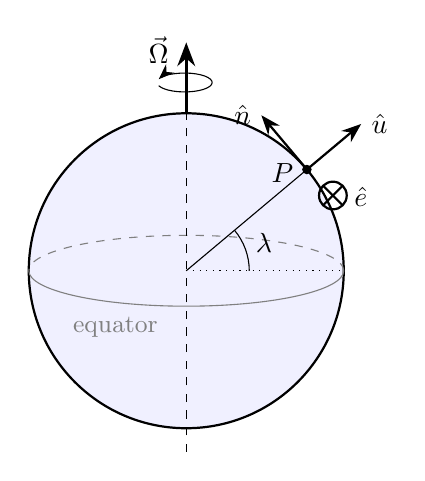
\begin{tikzpicture}[scale=1.0]
    \def\R{2}
    \def\lat{40}

    % Earth
    \filldraw[fill=blue!6, thick] (0,0) circle (\R);
    % Equator (front solid, back dashed)
    \draw[gray] (-\R,0) arc (180:360:{\R} and {0.45});
    \draw[gray, dashed] (\R,0) arc (0:180:{\R} and {0.45});
    \node[gray, font=\small] at (-0.9,-0.72) {equator};

    % Rotation axis and angular velocity
    \draw[dashed] (0,-\R-0.3) -- (0,\R);
    \draw[-{Stealth[length=3mm]}, very thick] (0,\R) -- (0,\R+0.9);
    \node[left] at (-0.1,\R+0.8) {$\vec{\Omega}$};
    % rotation sense
    \draw[-{Stealth[length=2mm]}] (-0.35,\R+0.35) arc (200:520:{0.35} and {0.12});

    % Site P at latitude lambda
    \coordinate (C) at (0,0);
    \coordinate (P) at ({\R*cos(\lat)},{\R*sin(\lat)});
    \draw (C) -- (P);
    \draw[dotted] (C) -- (\R,0);
    \draw (0.8,0) arc (0:\lat:0.8);
    \node at ({1.05*cos(\lat/2)},{1.05*sin(\lat/2)}) {$\lambda$};
    \filldraw (P) circle (1.5pt);
    \node[left] at ($(P)+(-0.05,-0.05)$) {$P$};

    % Local ENU axes at P
    \draw[-{Stealth[length=2.5mm]}, thick] (P) -- ++({0.9*cos(\lat)},{0.9*sin(\lat)}) node[right] {$\uhat$};
    \draw[-{Stealth[length=2.5mm]}, thick] (P) -- ++({-0.9*sin(\lat)},{0.9*cos(\lat)}) node[left] {$\nhat$};
    \draw[thick] ($(P)+(0.33,-0.33)$) circle (5pt);
    \draw[thick] ($(P)+(0.33,-0.33)+(-3.5pt,-3.5pt)$) -- ($(P)+(0.33,-0.33)+(3.5pt,3.5pt)$);
    \draw[thick] ($(P)+(0.33,-0.33)+(-3.5pt,3.5pt)$) -- ($(P)+(0.33,-0.33)+(3.5pt,-3.5pt)$);
    \node[right] at ($(P)+(0.48,-0.35)$) {$\ehat$};
\end{tikzpicture}
\hspace{1.2cm}
% ---------------- Right panel: pendulum in the ENU frame ----------------
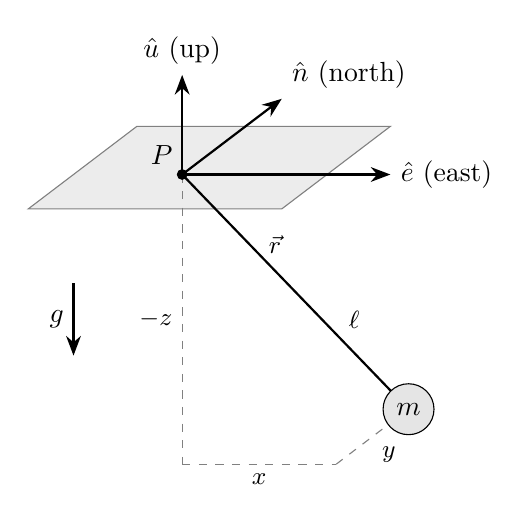
\begin{tikzpicture}[scale=1.15,
    x={(1cm,0cm)}, y={(0.5cm,0.38cm)}, z={(0cm,1cm)}]
    % 3D coordinates (x,y,z) = (east, north, up); pivot O at the origin
    \def\bx{1.7}
    \def\by{1.6}
    \def\bz{-3.2}

    % Ceiling plane at pivot level
    \filldraw[fill=gray!15, draw=gray] (-1.2,-1,0) -- (1.6,-1,0) -- (1.6,1.4,0) -- (-1.2,1.4,0) -- cycle;

    % ENU axes at the pivot
    \draw[-{Stealth[length=2.5mm]}, thick] (0,0,0) -- (2.3,0,0) node[right] {$\ehat$ (east)};
    \draw[-{Stealth[length=2.5mm]}, thick] (0,0,0) -- (0,2.2,0) node[above right] {$\nhat$ (north)};
    \draw[-{Stealth[length=2.5mm]}, thick] (0,0,0) -- (0,0,1.1) node[above] {$\uhat$ (up)};

    % Coordinate box: O -> (0,0,z) -> (x,0,z) -> (x,y,z)
    \draw[dashed, gray] (0,0,0) -- (0,0,\bz);
    \draw[dashed, gray] (0,0,\bz) -- (\bx,0,\bz);
    \draw[dashed, gray] (\bx,0,\bz) -- (\bx,\by,\bz);
    \node[left, font=\small] at (0,0,{\bz/2}) {$-z$};
    \node[below, font=\small] at ({\bx/2},0,\bz) {$x$};
    \node[below right, font=\small] at (\bx,{\by/2},\bz) {$y$};

    % String and bob
    \draw[thick] (0,0,0) -- (\bx,\by,\bz);
    \filldraw (0,0,0) circle (1.5pt);
    \node[above left] at (0,0,0) {$P$};
    \filldraw[fill=gray!20] (\bx,\by,\bz) circle (8pt);
    \node at (\bx,\by,\bz) {$m$};
    \node[font=\small] at ({0.62*\bx+0.35},{0.62*\by},{0.62*\bz}) {$\ell$};

    % Position vector label
    \node[font=\small, right] at ({0.3*\bx+0.1},{0.3*\by},{0.3*\bz}) {$\vec{r}$};

    % Gravity
    \draw[-{Stealth[length=2.5mm]}, thick] (-1.2,0,-1.2) -- (-1.2,0,-2.0);
    \node[left] at (-1.2,0,-1.6) {$g$};
\end{tikzpicture}
\caption{Left: a point $P$ fixed to the Earth's surface at latitude $\lambda$, with local east--north--up unit vectors $(\ehat,\nhat,\uhat)$ ($\ehat$ points into the page). Right: the pendulum, with its pivot at $P$, in the local ENU frame.}
\label{fig:foucault}
\end{figure}

\noindent A Foucault pendulum consists of a point mass $m$ hanging from a massless cable of length $\ell$. The pivot $P$ is fixed to the surface of the Earth at latitude $\lambda$, and the Earth rotates with constant angular velocity $\vec{\Omega}$ (magnitude $\Omega$) about its polar axis. We describe the motion of the mass in the \emph{local}, Earth-fixed east--north--up (ENU) frame with origin at the pivot:
\[
\vec{r} = x\,\ehat + y\,\nhat + z\,\uhat,
\]
so the mass hangs below the pivot with $z<0$, and gravity acts in the $-\uhat$ direction. Note that the ENU frame rotates with the Earth, so it is \emph{not} an inertial frame. We'll make the following assumptions throughout this assignment:
\begin{itemize}
    \item The system is frictionless with no energy loss.
    \item The pivot $P$ itself moves in a circle as the Earth turns. You may ignore this: its only effect is a tiny, constant correction to the magnitude and direction of the local gravitational acceleration, which we absorb into the definition of $g$ and the ``up'' direction $\uhat$.
    \item The cable stays taut, so $x^2+y^2+z^2=\ell^2$ at all times.
\end{itemize}

\section{Deriving Equations of Motion}

\begin{enumerate}[label=(\alph*)]
    \item \textbf{Energies:} First, express the Earth's angular velocity $\vec{\Omega}$ in ENU components in terms of $\Omega$ and $\lambda$ (consistent with Fig.~\ref{fig:foucault}). Then write the velocity of the mass as seen from an inertial frame. Remember that you can ignore the translational motion of $P$ relative to the Earth's center and simply account for its rotation. Use this to write the kinetic energy $T$ and the gravitational potential energy $U$ in terms of $x, y, z$ and their time derivatives.

    We'll use parameters $\Omega \approx 7.29\times10^{-5}$~rad/s, $\ell = 10$~m, and $g = 9.81$~m/s$^2$. Therefore,  $\mathcal{O}(\Omega^2)$ terms are small enough to ignore.

    \item \textbf{Eliminate the constraint:} Use the length constraint to write $z$ (and $\dot z$) as functions of $x$, $y$, $\dot x$, and $\dot y$. Be careful to choose the sign for $z$ consistent with Fig. 1. Substitute into $T$ and $U$ to obtain the Lagrangian $L(x,y,\dot x,\dot y)$ for a system with two generalized coordinates, $\bq = [x\;\; y]^T$.

    \item \textbf{Linearization via the Lagrangian:} Taylor expand the Lagrangian to \emph{second order} in the small quantities $x$, $y$, $\dot x$, $\dot y$ about the equilibrium $\bq=\dot{\bq}=\mathbf{0}$. Derive linear equations of motion from the quadratic Lagrangian and write them in the form
        \begin{equation} \label{ode}
        \bM\,\ddot{\bq} + \mathbf{C}\,\dot{\bq} + \mathbf{K}\,\bq = \mathbf{0},
        \end{equation}
        where $\bM$, $\mathbf{C}$, and $\mathbf{K}$ are constant $2\times2$ matrices. What special structure does $\mathbf{C}$ have?
\end{enumerate}

\section{Analyzing Precession}

The characteristic behavior of a Foucault pendulum is that the plane in which it swings slowly rotates (\emph{precesses}) relative to the ground. Let $\psi$ denote the angle of the swing plane, measured counterclockwise from $\ehat$ toward $\nhat$ when viewed from above.
 If we move into a frame that rotates at the (constant) precession rate $\dot{\psi}$, the dynamics should reduce to an ordinary (non-precessing) pendulum (i.e. the $\bf{C \, \dot{q}}$ term should drop out). Let's define the change of coordinates
	\begin{equation}
		\bq = \bf{R}(\psi) \tilde{q} ,
	\end{equation}
	where $\bf{R}$ is a rotation matrix and $\bf{\tilde{q}}$ is the pendulum's position in the rotating frame. Differentiate this expression twice to calculate $\bf{\ddot{q}}$, then plug it back into \eqref{ode} to derive a new ODE in terms of $\bf{\tilde{q}}$. \emph{Hint:} you may want to use the fact that $\Omega \ll \sqrt{g/\ell}$.
\begin{enumerate}[label=(\alph*)]
		\item By matching up terms, identify the precession rate $\dot{\psi}$.
        \item Does the swing plane rotate clockwise or counterclockwise when viewed from above in the northern hemisphere? What happens at the equator and at the North Pole?
        \item Compute the predicted precession period (in hours) at the latitude of MIT, $\lambda = 42.36^\circ$\,N. Use the \emph{sidereal} rotation rate of the Earth, $\Omega \approx 7.2921\times10^{-5}$~rad/s.
    \end{enumerate}
    

\section{Simulation}

Numerically integrate the equations of motion from Section 1(c) at $\lambda = 42.36^\circ$ with $\ell = 10$~m, $g = 9.81$~m/s$^2$, and $\Omega = 7.2921\times10^{-5}$~rad/s, using MATLAB (\texttt{ode45}) or Python (\texttt{scipy.integrate.\allowbreak solve\_ivp}). Release the pendulum from rest (relative to the ground) with the cable displaced $\theta_0 = 5^\circ$ from vertical toward the east. Simulate for at least one full precession period. This is several thousand swings, so you will need tight integration tolerances (e.g., relative and absolute tolerances of $10^{-10}$).
    \begin{itemize}
        \item  As a sanity check on your integrator, verify that the total energy of the system is conserved.
        \item Plot the precession angle $\psi$ versus time, along with your prediction from part 2(a) on the same axes. Fit a line to your simulated $\psi(t)$ and report the percent error between the measured and predicted precession rates. \emph{Hint:} compute $\psi$ once per swing period at the pendulum's point of maximum displacement. Make sure that angle wrap-around is properly handled.
\end{itemize}


\end{document}
